\section{Domande d'esame}
\begin{figure}[H]
    \centering  
    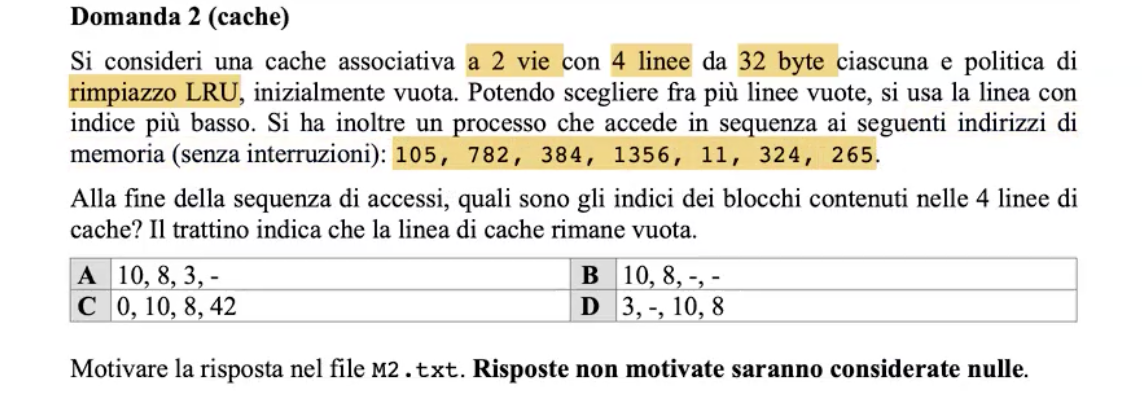
\includegraphics[width=0.9\linewidth]{../images/Domanda esame Controlli 1.png}
    \caption{Domande 1}
    %\label{label}
\end{figure}
\begin{figure}[H]
    \centering  
    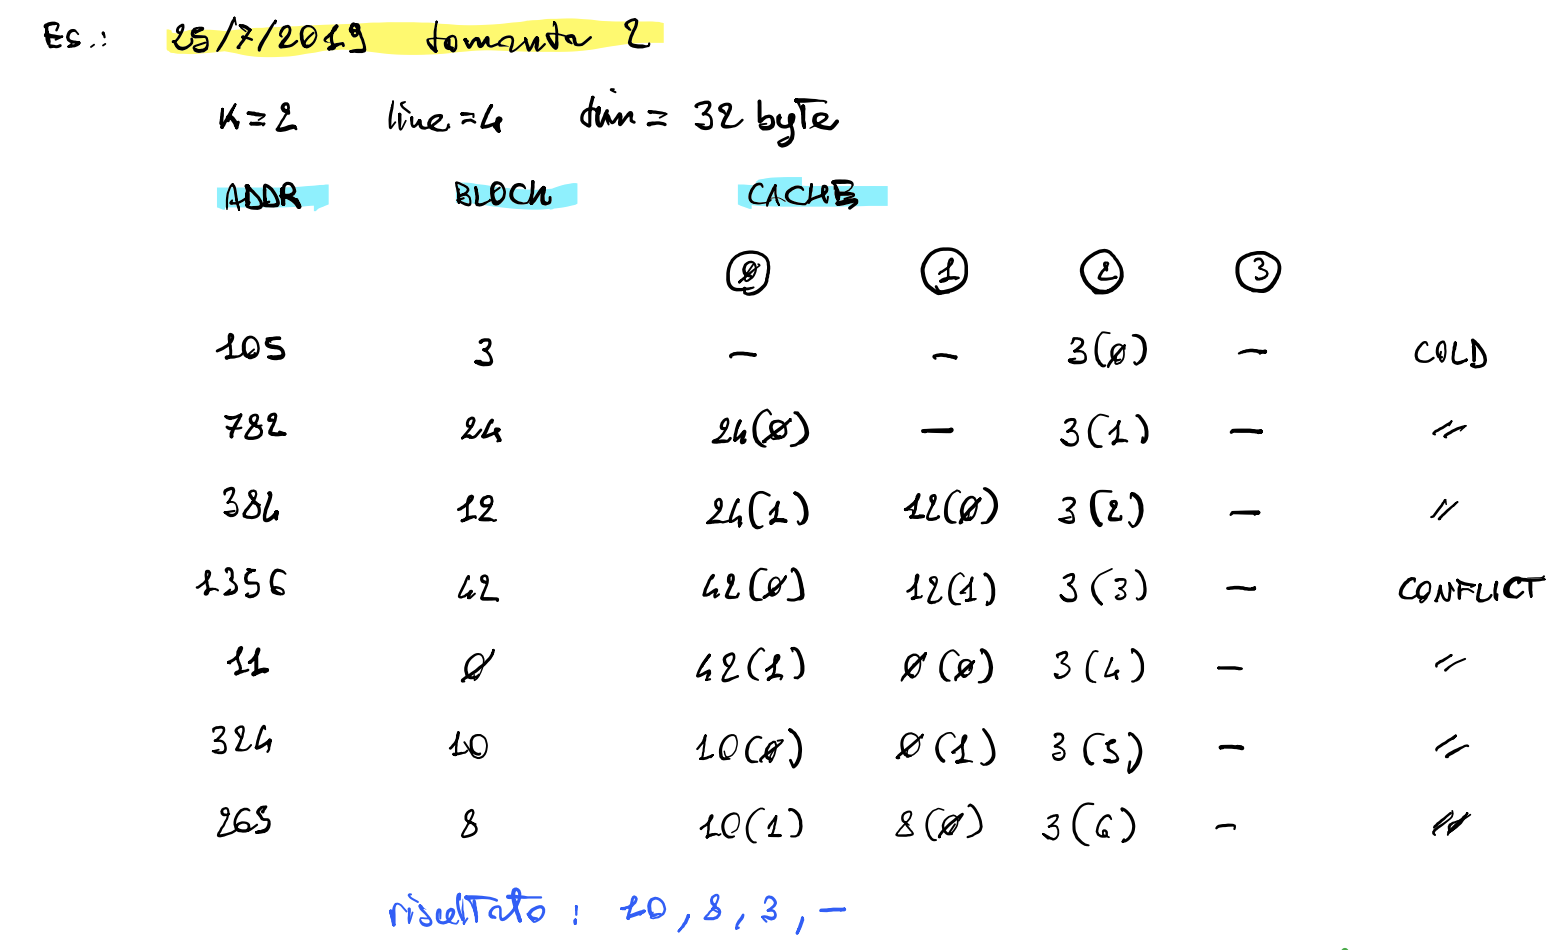
\includegraphics[width=0.9\linewidth]{../images/Eserizio Svolgimento 1.png }
    \caption{Svolgimento 1}
    %\label{label}
\end{figure}
\begin{figure}[H]
    \centering  
    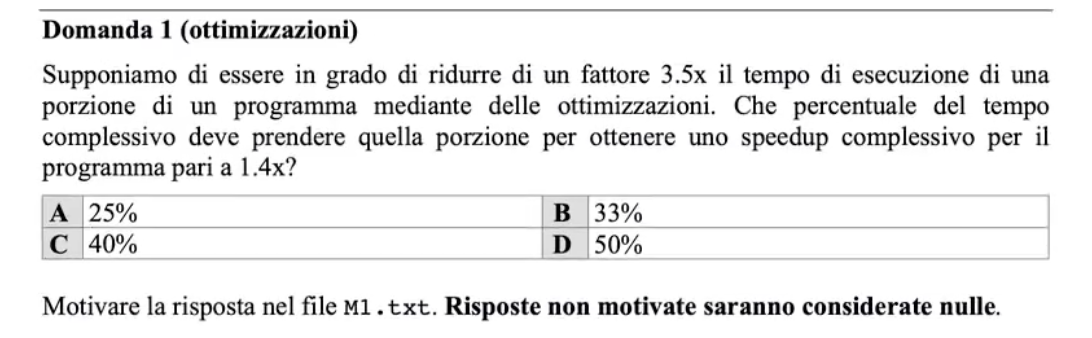
\includegraphics[width=0.9\linewidth]{../images/Domanda esame Controlli 2.png}
    \caption{Domande 2}
    %\label{label}
\end{figure}
\begin{figure}[H]
    \centering  
    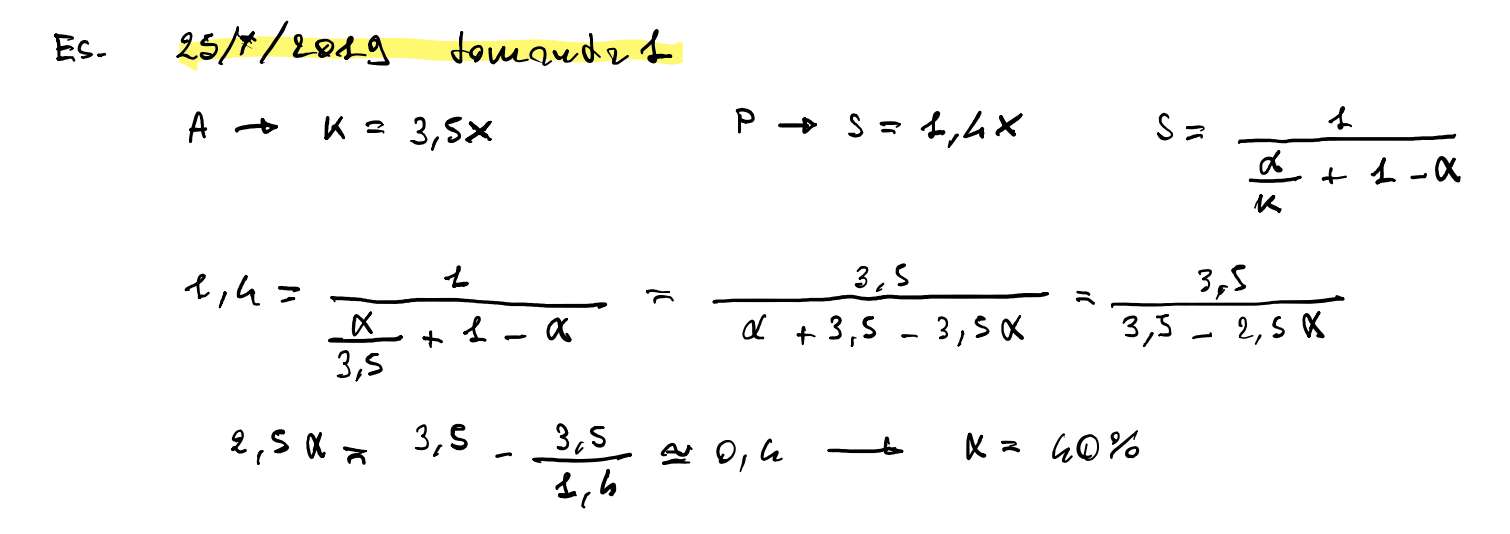
\includegraphics[width=0.9\linewidth]{../images/Eserizio Svolgimento 2.png }
    \caption{Svolgimento 2}
    %\label{label}
\end{figure}
\begin{figure}[H]
    \centering  
    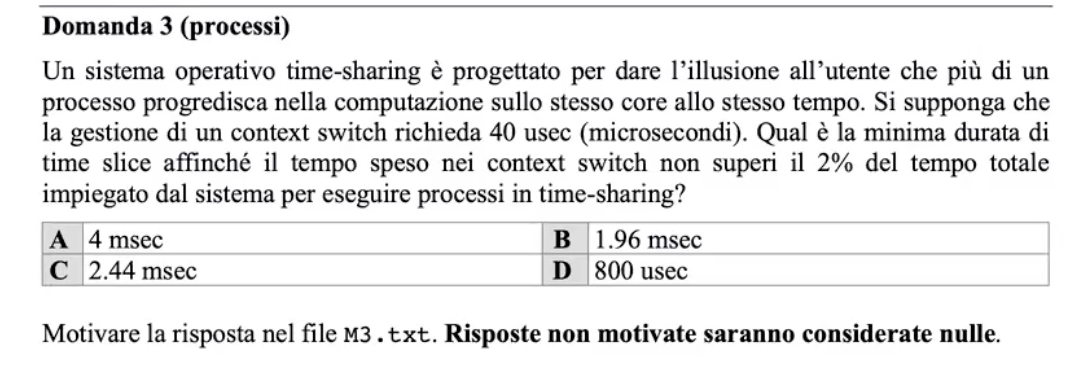
\includegraphics[width=0.9\linewidth]{../images/Domanda esame Controlli 3.png}
    \caption{Domande 3}
    %\label{label}
\end{figure}
\begin{figure}[H]
    \centering  
    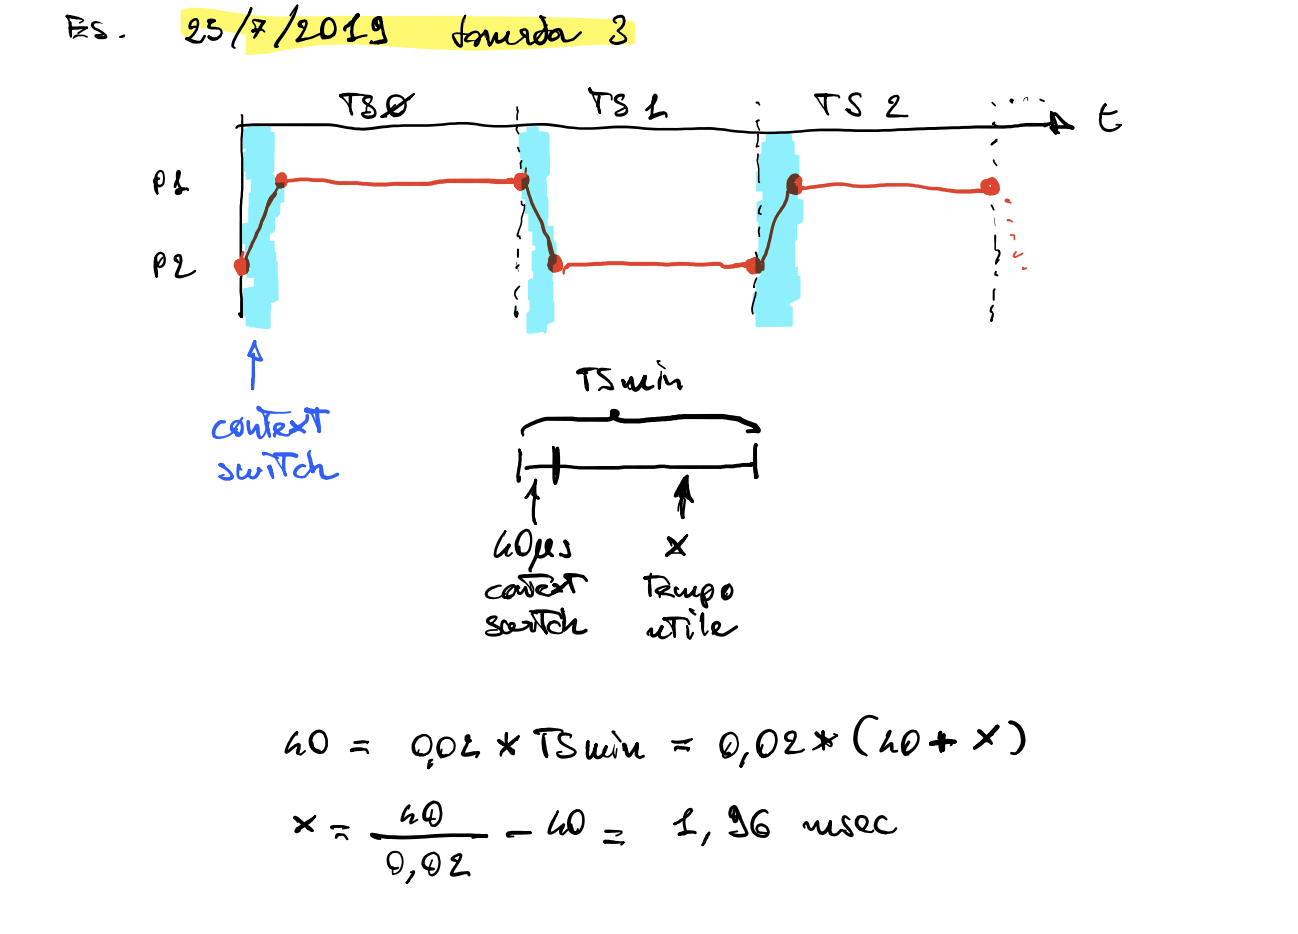
\includegraphics[width=0.9\linewidth]{../images/Eserizio Svolgimento 3.png }
    \caption{Svolgimento 3}
    %\label{label}
\end{figure}
\begin{figure}[H]
    \centering  
    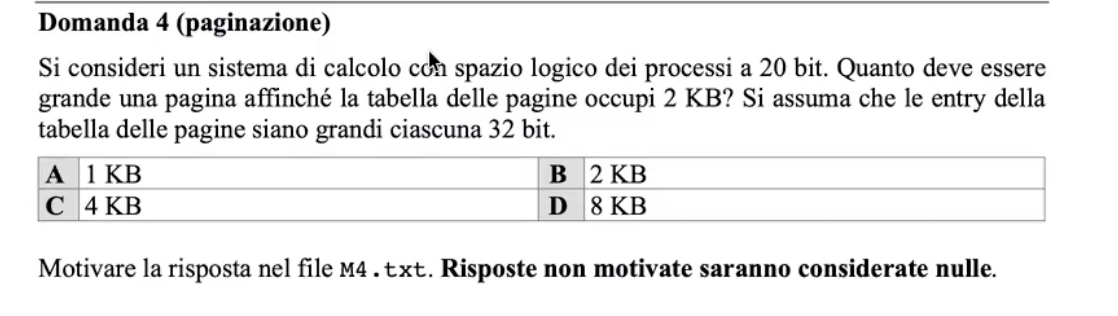
\includegraphics[width=0.9\linewidth]{../images/Domanda esame Controlli 4.png}
    \caption{Domande 4}
    %\label{label}
\end{figure}
\begin{figure}[H]
    \centering  
    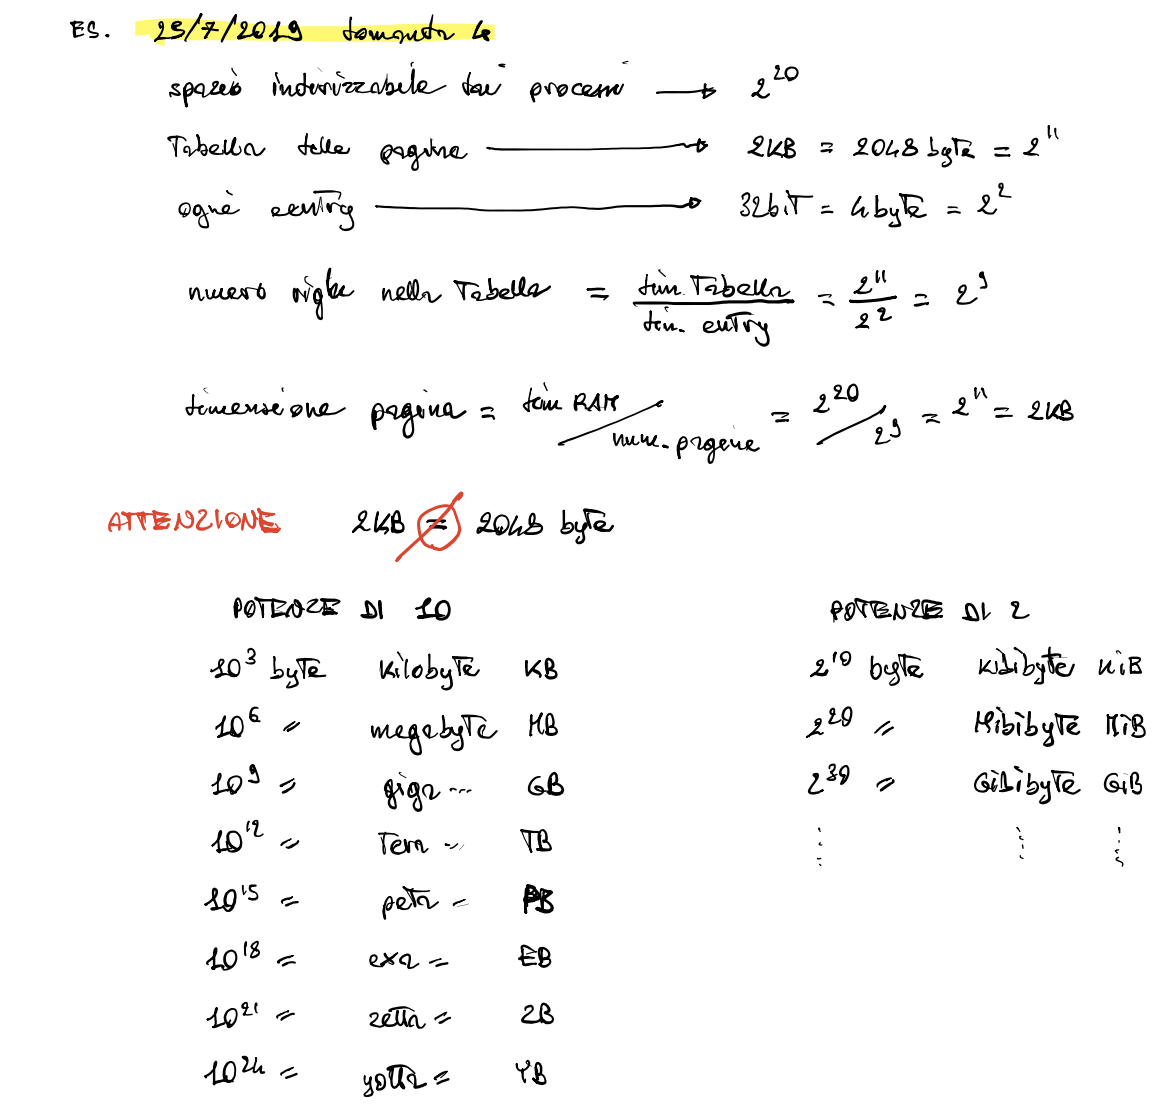
\includegraphics[width=0.9\linewidth]{../images/Eserizio Svolgimento 4.png }
    \caption{Svolgimento 4}
    %\label{label}
\end{figure}
\begin{figure}[H]
    \centering  
    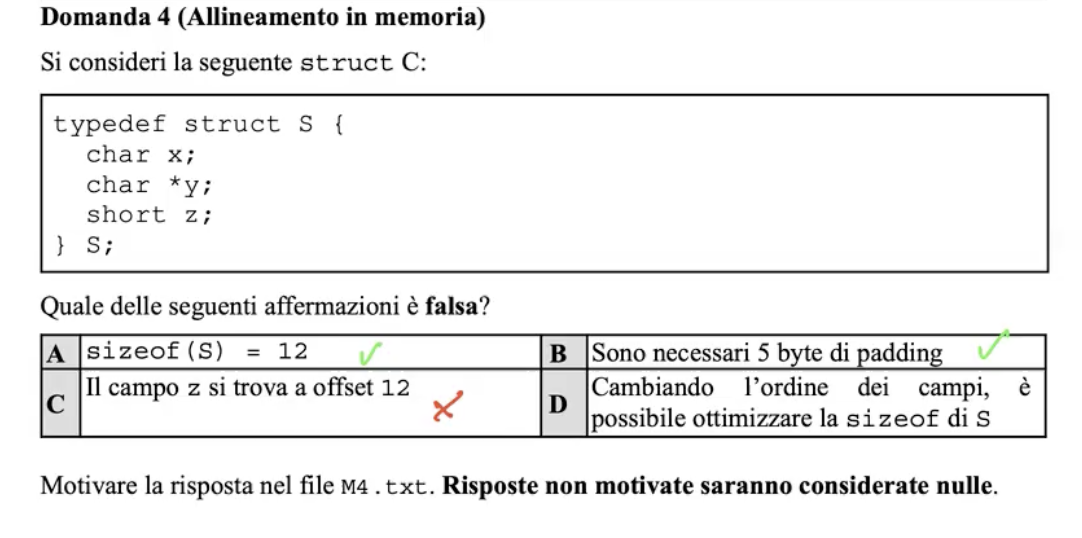
\includegraphics[width=0.9\linewidth]{../images/Domanda esame Controlli 5.png}
    \caption{Domande 5}
    %\label{label}
\end{figure}
\begin{figure}[H]
    \centering  
    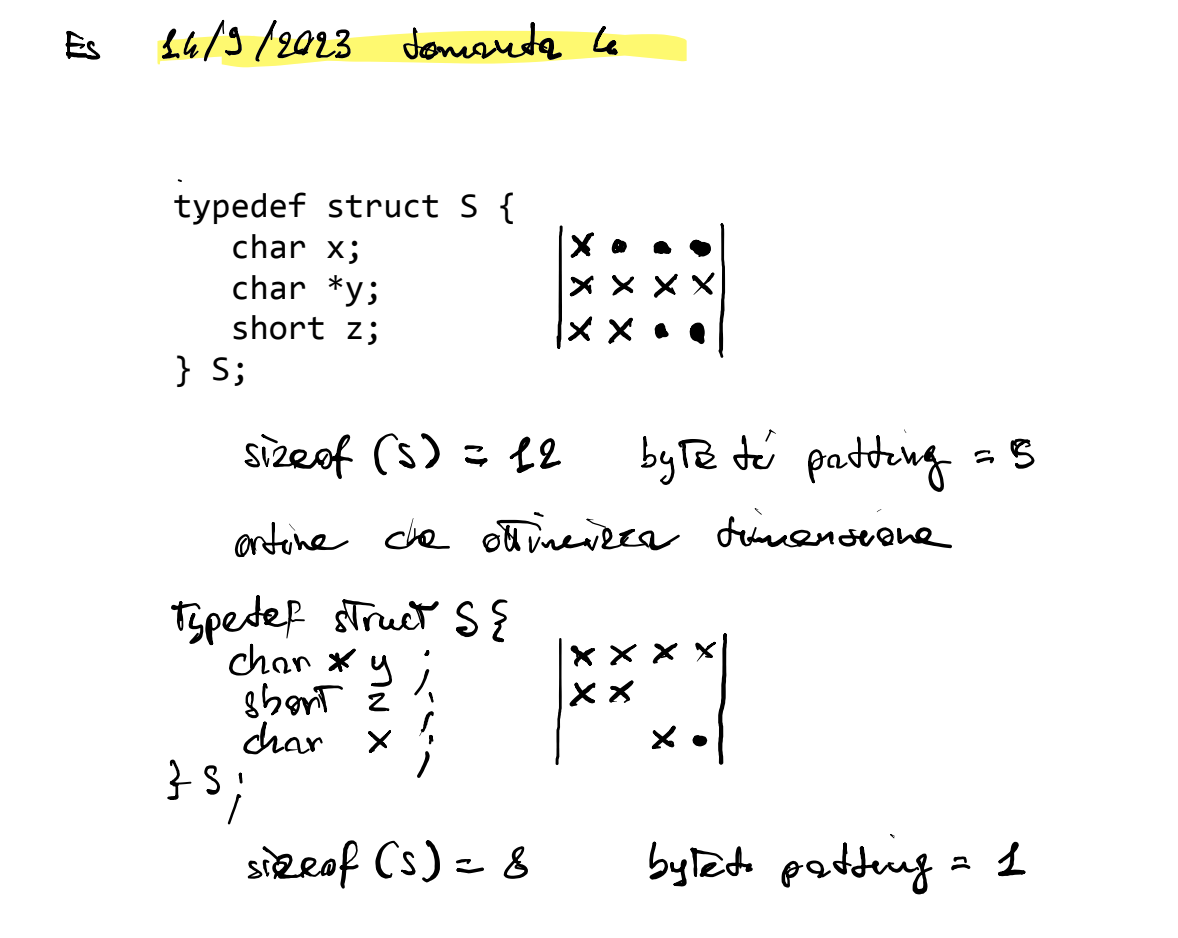
\includegraphics[width=0.9\linewidth]{../images/Eserizio Svolgimento 5.png }
    \caption{Svolgimento 5}
    %\label{label}
\end{figure}\begin{figure}[H]
    \centering  
    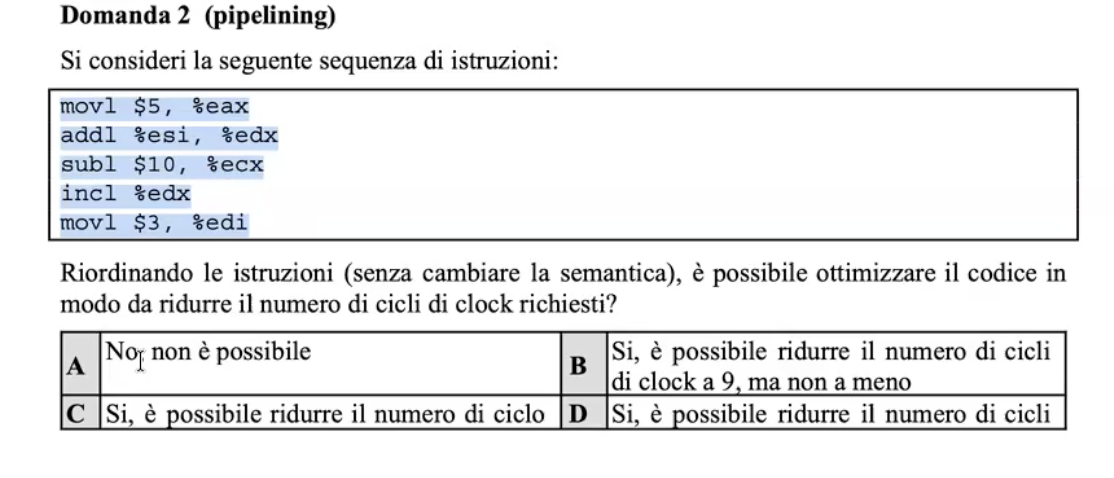
\includegraphics[width=0.9\linewidth]{../images/Domanda esame Controlli 6.png}
    \caption{Domande 6}
    %\label{label}
\end{figure}
\begin{figure}[H]
    \centering  
    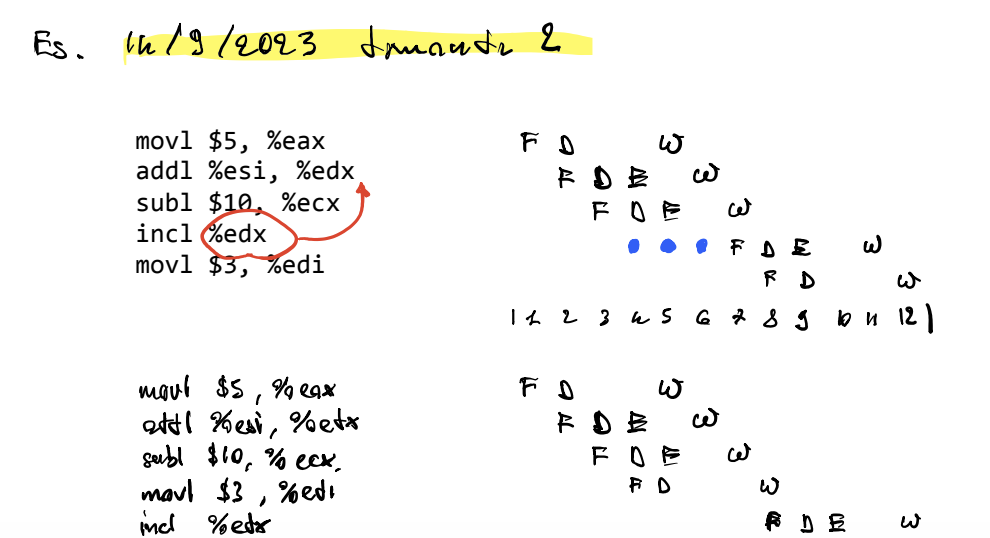
\includegraphics[width=0.9\linewidth]{../images/Eserizio Svolgimento 6.png }
    \caption{Svolgimento 6}
    %\label{label}
\end{figure}